\providecommand{\main}{../../..}

\documentclass[\main/main.tex]{subfiles}

\providecommand{\Images}{\main/Figures/intro_seg}
\providecommand{\Figures}{\main/Figures}


\begin{document}
            
\section{Présentation de différentes stratégies de segmentation automatique}

%
La segmentation d'image consiste à grouper des pixels afin d'extraire une information de l'image, par exemple identifier une ou plusieurs régions d'intérêt.
%
Dans le cadre d'imageries de tissus biologiques,
ces régions d'intérêt peuvent être un organe entier ou une sous\hyp{}région de cet organe~\cite{early_2018,liu_2020,gupta_2018},
une anomalie dans une structure~\cite{wadhwa_2019,huang_2019,ruikar_2019}
ou un caractère particulier~\cite{teixid_2019,hinfray_2018} .
%
L'approche la plus simple de segmentation consiste à manuellement annoter l'image que l'on souhaite étudier pixel par pixel.
%
Cette approche permet en principe d'avoir le résultat le plus précis,
mais c'est une procédure extrêmement longue, ce qui rend son emploi incompatible avec le traitement d'un grand nombre d'image.
%
Il est interminale de définir de façon précise manuellement les limites d'une région, et la segmentation manuelle présente de fort risque de biais inter et intra\hyp{}individuels~\cite{heye_2013}.
%
Les biais intra\hyp{}individuels peuvent être limité par l'utilisation d'outil de segmentation semi\hyp{}manuels~\cite{berg_2019,benenson_2019} qui permettent à l'utilisateur de définir un ensemble de paramètres qui seront ensuite appliqués à toutes les segmentations manuelles effectués par cet utilisateur.
%
La segmentation manuelle reste malgré tout une procédure de choix dans l'évaluation d'algorithmes de segmentation.
%
Pour accélérer la segmentation et le rendre plus précise, il est possible de mettre en place des algorithmes de segmentations automatiques.
%
Nous allons donc maintenant faire un état de l'art de différentes approches de la segmentations automatiques, et aussi exposer les limites inhérentes à ces algorithmes.

    \subsection{Le seuillage, une approche simple mais insuffisante}
    
%
Le seuillage est une procédure d'étiquetage des pixels en deux classes en fonction des valeurs de gris des pixels. Elle consiste à conserver tous les pixels supérieurs à une valeur définie. De par sa simplicité, elle a été une des premières stratégie de segmentation automatique~\cite{sakai_1969,otsu_1979}.
%
De plus, il s'agit d'une procédure régulièrement utilisé dans l'initiation de segmentations manuelles.
%
Cette méthode est applicable dans de nombreux cas: par exemple pour estimer la radio\hyp{}densité d'un tissu dans le cas d'image de scanner,ou pour mettre en avanr des régions d'intérêt par un marqueur, tel qu'un anticorps lié à un fluorophore.
%
Au fur et à mesure du développement des méthodes de segmentations automatiques, les seuillages se sont diversifiés.
Nous allons donc maintenant présenter diverses approches de seuillages présentes dans la littérature.

% Seuil choisi à priori
L'approche la plus simple est l'emploi d'une valeur de seuil définie à priori~\cite{hinfray_2018}.
%
De nombreux outils de visualisation d'images permettent d'effectuer rapidement ce type ces procédures et de les automatiser, par exemple avec des macros ImageJ.
%
Cependant, la détermination de la valeur seuil est un point limitant de cette méthode, du fait de la variabilité des niveaux de gris entre acquisitions, en particulier si les dispositifs d'imagerie ne sont pas calibrés.
%
Si les images ne sont pas saturées , le même histogramme de valeur de gris pour une modalité donnée est obtenu quelque soit l'opérateur ou l'appareil employé.
%
Différentes approches de seuillage utilisent cet histogramme pour choisir la valeur seuil.
%
La solution la plus simple consiste à ne conserver qu'une proportion de pixels en choisissant la valeur seuil de manière à ce que le nombre de pixels ayant une valeur supérieure à ce seuil soit équivalent à la proportion de pixels que l'on souhaite conserver.
%
Cette méthode présente toutefois le défaut de devoir prédéfinir la surface totale de la segmentation ce qui peut induire des défauts importants de segmentations si la taille ou la forme des objets varient.
%
Il est donc souhaitable de tenter de définir automatiquement la valeur seuil, une des premières approches de ce type ayant été proposé par \textsc{Nobuyuki Otsu}~\cite{otsu_1979}.
%
Considérons une image, scindée en deux classes de valeurs de gris, avec une variance de valeurs de gris inter\hyp{}groupe différente. En utilisant l'histogramme des valeurs de gris, il est possible de définir une valeur de gris qui permet de maximiser la variance inter\hyp{}groupe.
%
Cette approche est facilement généralisable à la segmentation de plusieurs classes de pixels. Pour une segmentation en $n$ classes, il suffit alors de chercher les $n-1$ critères permettant de maximiser les variances entre chaque groupes~\cite{kugler_2019,ibrahim_2020,huang_2020}.

%% Défauts
%
La simplicité des algorithmes de seuillage les rend présents dans de nombreuses algorithmes de segmentations automatiques alors que  ces approches présentent de nombreux défauts.
%
Tout d'abord, ces approches considèrent que l'image est séparable en région ayant des valeurs de gris proches. Il est cependant possible qu'une région d'intérêt ne soit pas uniforme, et présente en son sein une grande variété de valeurs de gris. Si les transitions ne sont pas abruptes, l'utilisation d'algorithmes de seuillage devient alors impossible.
Ensuite, il s'agit pour la plupart d'algorithmes appliqués sur l'ensemble de l'image ce qui peut entraîner de nombreuses complications.
%
Ne prenant pas en compte le voisinage de chaque pixel, ces algorithmes considèrent indifféremment un pixel se trouvant bien au centre de la région segmentée ou à l'extérieur, isolé sur un fond plus sombre par exemple. Cela mène à des isolats de pixel au sein d'une région.
%
Enfin, ces procédures n'étant basées que sur la séparation de l'image en deux classes de valeurs de gris, il n'est pas possible de segmenter des régions ayant des valeurs de gris similaires mais séparées par un changement de textures ou séparées par un changement local d'intensité lumineuse.
%%
Il faut donc mettre en place un ensemble de filtre permettant de corriger les images avant de les seuiller. La morphologie mathématique apporte un certain nombre de ces filtres, ainsi que ses propres procédures de segmentation.
%
Nous allons donc maintenant voir comment la morphologie mathématique peut permettre d'améliorer la segmentation automatique d'images.

    \subsection{La morphologie mathématique améliore la précision des segmentations}
    
%
La morphologie mathématique est un théorie mathématique principalement développée afin de mettre au point des procédures d'analyse d'image.
%
Deux opérateurs de bases sont employés, l'érosion et la dilatation.
%
Pour une image en niveaux de gris, il s'agit de calculer respectivement le minimum ou le maximum au voisinage de chaque pixel (Voir \autoref{fig:morpho:operateurs}).
%
Le voisinage concerné est appelé élément structurant, et peut avoir un grand nombre de formes.
%
L'utilisation d'une forme particulière peut alors permettre de révéler une structure particulière dans une image.
%
Par exemple, une érosion par un ensemble de lignes tournant autour du point d'intérêt peut permettre de faire disparaître des structures linéaires.
%
Un troisième opérateur est le filtre de rang, qui consiste à conserver pour chaque pixel la $n$\textsuperscript{ième} valeur du voisinage, $n$ étant le rang de l'élément.
%
L'exemple de filtre de rang le plus connu est le filtre médian, qui remplace chaque pixel par la valeur médiane au sein  de l'élément structurant choisi.

\begin{figure}[h]
    \centering
    \begin{subfigure}[b]{0.30\textwidth}
       \caption{
       Image d'origine
            }
       \centering 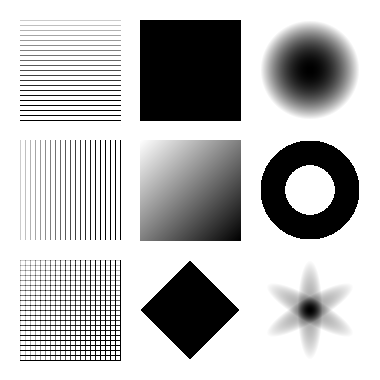
\includegraphics[width=\textwidth]{\Images/operators_reference.png}
    \end{subfigure}
    \begin{subfigure}[b]{0.30\textwidth}
       \caption{
            Après dilatation
            }
       \centering 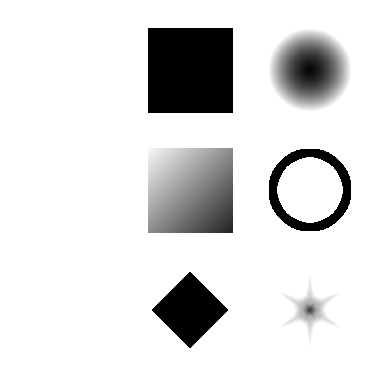
\includegraphics[width=\textwidth]{\Images/operators_reference_dilated_disk.png}
    \end{subfigure}
    \begin{subfigure}[b]{0.30\textwidth}
       \caption{
            Après erosion
            }
       \centering 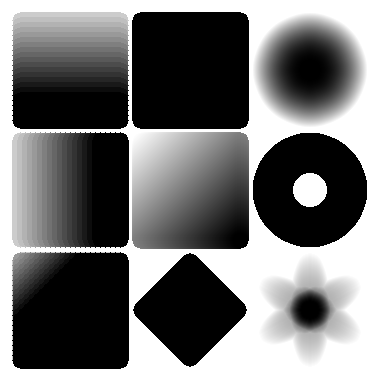
\includegraphics[width=\textwidth]{\Images/operators_reference_eroded_disk.png}
    \end{subfigure}
    \caption{
        \label{fig:morpho:operateurs}
        Exemple d'application d'une érosion et d'une dilatation.\newline
        La dilatation consistant à conserver pour chaque pixel le maximum local se trouvant au sein du voisinage, elle va avoir pour effet d'étaler les blancs. A l'inverse, l'érosion va étaler les noirs.
    }
    
\end{figure}

\begin{figure}[h]
    \centering
    \begin{subfigure}[b]{0.45\textwidth}
       \caption{
       Image d'origine
            }
       \centering 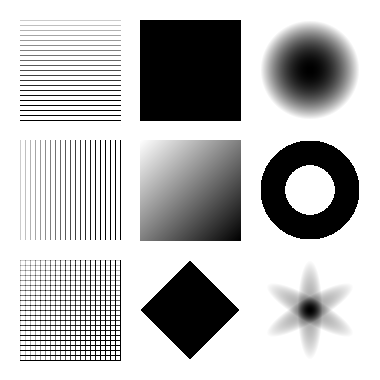
\includegraphics[width=\textwidth]{\Images/operators_reference.png}
    \end{subfigure}
    \begin{subfigure}[b]{0.45\textwidth}
       \caption{
       Cercle
            }
       \centering 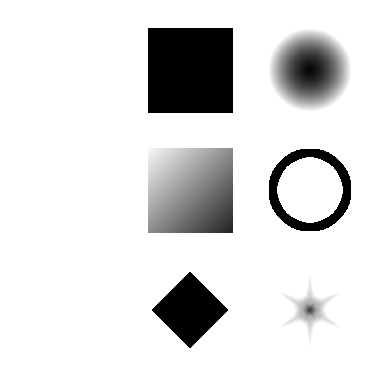
\includegraphics[width=\textwidth]{\Images/operators_reference_dilated_disk.png}
    \end{subfigure}
    \begin{subfigure}[b]{0.45\textwidth}
       \caption{
       ligne horizontale
            }
       \centering 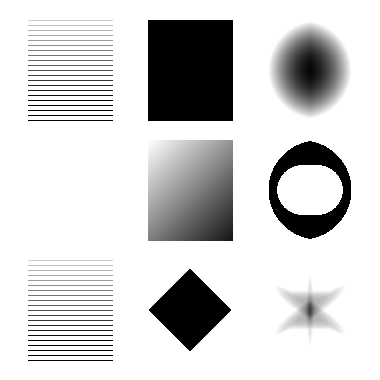
\includegraphics[width=\textwidth]{\Images/operators_reference_dilated_line_0.png}
    \end{subfigure}
    \begin{subfigure}[b]{0.45\textwidth}
       \caption{
       Ellipse
            }
       \centering 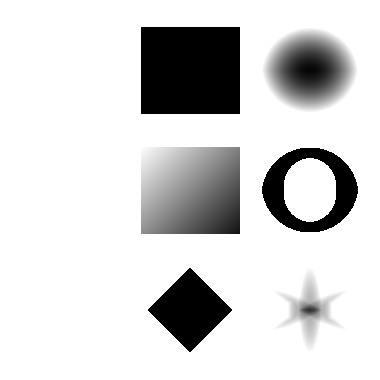
\includegraphics[width=\textwidth]{\Images/operators_reference_dilated_ellips_0.png}
    \end{subfigure}
    \caption{
        \label{fig:morpho:operateurs}
        Exemple d'application d'une dilatation avec différentes formes d'éléments structurants, comme indiquant au dessus de chaque panneau.
        \newline
        Le choix de l'élément structurant utilisé à un impact important sur le résultat.
        L'utilisation d'éléments structurants circulaires ou elliptiques ne permet pas de conserver les lignes.
        L'utilisation de ligne horizontale fera disparaître toute ligne n'ayant pas la même orientation.
    }
    
\end{figure}
%
%
En combinant l'érosion et la dilatation, deux opérateurs se rajoutent.
%
La succession d'une érosion puis d'une dilatation utilisant le même élément structurant
est appelé une ouverture
(voir \autoref{fig:ouverture}).
%
Cette opérateur permet de supprimer des objets de petites tailles ou des structures fines.
%
A l'inverse, la succession d'une dilatation puis d'une érosion est appelée une fermeture
(voir \autoref{fig:fermeture}).
%
A l'inverse de l'ouverture, cet opérateur permet de remplir des aires et permet de joindre des éléments proches entre eux.
%
L'ouverture, la fermeture et le filtre de rang sont ainsi des outils de choix pour le pré\hyp{}traitement d'images, en permettant d'apporter une cohérence topographique à l'image que l'on veut étudier).


\begin{figure}[h]
    \centering
    \begin{subfigure}[b]{0.30\textwidth}
       \caption{
       Image d'origine
            }
       \centering 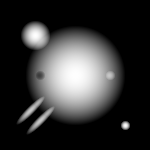
\includegraphics[width=\textwidth]{\Images/fantome.png}
    \end{subfigure}
    \begin{subfigure}[b]{0.30\textwidth}
       \caption{
        \label{fig:ouverture}
            Ouverture
            }
       \centering 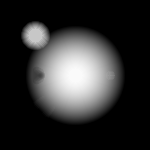
\includegraphics[width=\textwidth]{\Images/opened.png}
    \end{subfigure}
    \begin{subfigure}[b]{0.30\textwidth}
       \caption{
        \label{fig:fermeture}
            Fermeture
            }
       \centering 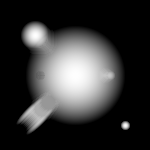
\includegraphics[width=\textwidth]{\Images/closed.png}
    \end{subfigure}
    \caption{
        Exemple d'application d'une ouverture et d'une fermeture.
        \newline
        L'ouverture permet de supprimer les éléments fins ou isolés.
        La fermeture permet de relier deux régions ou de supprimer des zones sombres.
        %
        En lissant les images en fonction du voisinage de chaque pixel, ces opérateurs améliore les segmentations par seuilage
    }
    
\end{figure}
%
Grâce à ces deux opérateurs, il est possible de définir deux transformations, les chapeaux haut-de-forme blanc et noir.
%
Le chapeau haut-de-forme blanc consiste en la soustraction d'une ouverture à l'image d'origine, alors que le chapeau haut-de-forme noir est la soustraction de l'image d'origine à une fermeture de cette image.
%
L'utilisation du chapeau haut-de-forme blanc permet la mise en évidence de régions ayant une forte intensité dans une zone restreinte ou ayant une forme particulière (voir \autoref{fig:tophat:blanc}).
%
A l'inverse, le chapeau haut-de-forme noir permet la mise en évidence de la proximité entre deux régions, ou la délimitation entre deux objets clairs (voir \autoref{fig:tophat:noir}).
%
Enfin, une dernière transformation est le gradient morphologique.
%
Calculé comme la soustraction d'une érosion à une dilatation d'une image,
le gradient morphologique permet de connaître l'évolution des valeurs de gris en chaque point de l'image.

\begin{figure}[h]
    \centering
    \begin{subfigure}[b]{0.30\textwidth}
       \caption{
       Image d'origine
            }
       \centering 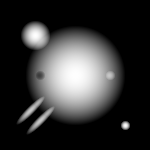
\includegraphics[width=\textwidth]{\Images/fantome.png}
    \end{subfigure}
    \begin{subfigure}[b]{0.30\textwidth}
       \caption{
       \label{fig:tophat:blanc}
            Chapeau haut-de-forme blanc
            }
       \centering 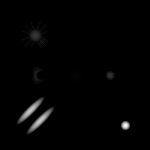
\includegraphics[width=\textwidth]{\Images/tophat_blanc.png}
    \end{subfigure}
    \begin{subfigure}[b]{0.30\textwidth}
       \caption{
           \label{fig:tophat:noir}
            Chapeau haut-de-forme noir
            }
       \centering 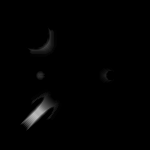
\includegraphics[width=\textwidth]{\Images/tophat_noir.png}
    \end{subfigure}
    \caption{
        Exemple de l'application d'un chapeau haut-de-forme.
        \newline
        Le chapeau haut\hyp{}de\hyp{}forme noir consiste à soustraire l'image d'origine à une fermeture de cette image. À l'inverse, le chapeau haut\hyp{}de\hyp{}forme blanc consiste à soustraire une ouverture à l'image d'origine.
        \newline
        Les chapeaux haut-de-forme permettent ainsi de détecter des éléments isolés,
        de mettre en avant des démarcations
        ou des régions situées entre deux objets proches.
        
    }
    
\end{figure}
%
Ces différents opérateurs et transformations sont régulièrement employés conjointement à une segmentation par seuillage,
que ce soit pour préparer le seuillage ou améliorer ses résultats~\cite{ilhan_2019,siri_2020,liu_2019}.

%
De plus, la morphologie mathématique propose un outil de segmentation, la ligne de partage des eaux~\cite{meyer_1994}.
%
En hydrologie, la ligne de partage des eaux est la ligne permettant de séparer différents bassins versants.
%
Ces lignes sont définis principalement en fonction de la topographie de la région étudiée, et suivent ainsi les crêtes topographiques.
%
En considérant les valeurs de gris d'une image comme décrivant la hauteur d'un pixel,
il est alors possible d'effectuer une analogie entre les deux systèmes.
%
Un algorithme de ligne de partage des eaux aura ainsi pour but de définir à quelle région appartient chaque pixel.
%
Pour définir son appartenance,
cet algorithme calculera à quel bassin versant appartient chaque pixel.
%
Pour cela, il utilise deux informations: une image qui servira de carte topographique, comme le gradient d'une image, et une liste de marqueurs qui serviront à définir les bassins versants(voir \autoref{fig:lpe:marqueurs}).
%
L'algorithme va alors attribuer à chaque pixel un label définissant à quel bassin versant il appartient (voir \autoref{fig:lpe:lines} et \autoref{fig:lpe:zones}).
%
Les lignes de partages des eaux seront alors l'ensemble des pixels pour lesquels deux bassins versants se sont rencontrés.
%
Cette approche permet ainsi de relier entre eux des régions présentant des valeurs de gris cohérentes afin de segmenter les régions par proximité topographiques des pixels~\cite{liang_2019,eschweiler_2019}.
%

\begin{figure}[h]
    \begin{subfigure}[b]{0.50\textwidth}
       \caption{
           \label{fig:lpe:marqueurs}
            Image d'origine
            }
       \centering 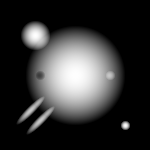
\includegraphics[width=\textwidth]{\Images/fantome.png}
    \end{subfigure}
    \begin{subfigure}[b]{0.5\textwidth}
       \caption{
           \label{fig:lpe:marqueurs}
           Gradient morphologique de l'image d'origine et marqueurs employés
            }
       \centering 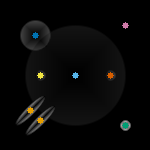
\includegraphics[width=\textwidth]{\Images/markers.png}
    \end{subfigure}
    \begin{subfigure}[b]{0.5\textwidth}
       \caption{
           \label{fig:lpe:lines}
           ligne\\ de partage des eaux
            }
       \centering 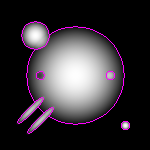
\includegraphics[width=\textwidth]{\Images/water_lines.png}
    \end{subfigure}
    \begin{subfigure}[b]{0.5\textwidth}
       \caption{
           \label{fig:lpe:zones}
            Bassins versants obtenus
            }
       \centering 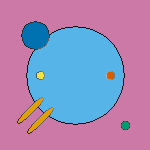
\includegraphics[width=\textwidth]{\Images/water_comp.png}
    \end{subfigure}
    \caption{
        Exemple d'application d'une \watershed{}.\newline
        La \watershed{} est calculée en utilisant le gradient morphologique de l'image d'origine et les marqueurs représentés en (b).
        Le gradient morphologique est un opérateur de morphologie mathématique consistant à soustraire une érosion à une dilatation de l'image d'entrée, ce qui permet de connaître l'évolution locale des niveaux de gris.
        La ligne de partage des eaux fourni ainsi une démarcation entre différentes bassins versants, ce qui fournit une segmentation une segmentation de l'image.
        
    }
    
\end{figure}

%
%
Cependant, la sélection des marqueurs permettant l'initialisation du calcul de lignes de partage des eaux constitue une limite de cette méthode.
%
En effet, l'utilisation d'un trop grand nombre de points peut amener à un découpage en un trop grand nombre de parties différentes (voir \autoref{fig:watershed:errors:quantite}).
%
De plus, un marqueur absent ou mal positionné induira une mauvaise segmentation de la région d'intérêt (voir \autoref{fig:watershed:errors:position}).

\begin{figure}[h]
    \begin{subfigure}[b]{\textwidth}
       \caption{
           \label{fig:watershed:errors:quantite}
            Trop grand nombre de marqueurs
            }
       \centering 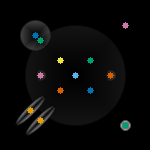
\includegraphics[width=0.30\textwidth]{\Images/markers_too_much.png} 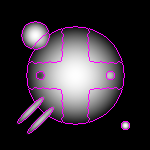
\includegraphics[width=0.30\textwidth]{\Images/water_without_markers_lines.png}
       \centering 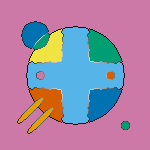
\includegraphics[width=0.30\textwidth]{\Images/water_too_much.png}
    \end{subfigure}
    \begin{subfigure}[b]{\textwidth}
       \caption{
           \label{fig:watershed:errors:position}
            Marqueurs mal placés ou absents
            }
       \centering 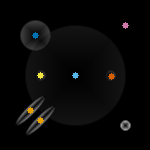
\includegraphics[width=0.30\textwidth]{\Images/markers_wrong.png} 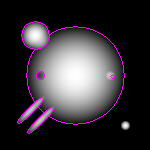
\includegraphics[width=0.30\textwidth]{\Images/water_wrong_markers_lines.png}
       \centering 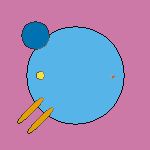
\includegraphics[width=0.30\textwidth]{\Images/water_wrong_markers.png}
       \centering
    \end{subfigure}
    \caption{
        Exemple de marqueurs entraînant des erreurs de segmentation.\newline
        Un trop grand nombre de classes de marqueurs va entraîner un sur\hyp{}découpage, alors qu'un mauvais placement des marqueurs peut mener à omettre certains éléments ou mener à de mauvais définitions de la ligne de partage des eaux.
    }
    
\end{figure}

%
En plus d'une forte sensibilité aux paramètres fournis, ces algorithmes sont pour la plupart relativement lents.
%
Ils ont ainsi été remplacés au cours de la dernière décennie par des algorithmes utilisant les réseaux de neurones profonds.

    \subsection{Une approche émergente, la segmentations par réseaux de neurones profonds}

% % Principe théorique
%
L'apprentissage par réseau de neurones est une technique de classification basée sur une analogie avec une vision simplifié du fonctionnement du cerveau.
%
Un ensemble de signaux interagit avec une première couche de neurones.
%
Chaque neurone de cette première couche va étudier ce signal, et émettre un signal répondant à sa fonction d'activation.
%
Ces signaux vont alors exciter ou inhiber une seconde couche de neurones, qui vont émettre à leur tour un signal répondant à la fonction d'activation choisi.
%
Les signaux vont ensuite être propagés vers les couches plus profondes jusqu'à atteindre la dernière couche de neurones, qui fournira le résultat désiré.
%
Cependant, pour chaque neurone, les signaux reçus doivent être pondérés afin de faire réagir chaque neurone d'une même couche différemment.
%
L'étape d'apprentissage du réseau de neurones consiste ainsi à faire varier ces poids pour que les résultats du réseau de neurones convergent vers une situation d'équilibre donnant les meilleurs résultats pour la classification des signaux d'entrée.
%
La profondeur du réseau de neurones est alors défini par le nombre de couches employé.
%
Une fois entraînés, ces réseaux de neurones permettent d'obtenir rapidement une classification efficace des signaux fournis.

%%
%
Les première utilisation de l'apprentissage de réseaux de neurones profonds pour l'analyse d'images a été la classification d'image en différentes classes~\cite{lecun_1989,krizhevsky_2012,Simonyan_2014}.
%
L'évolution des systèmes informatiques durant la dernière décennies ayant permis d'effectuer des réseaux de neurones de plus en plus profonds et de plus en plus peuplés, il a été possible de transformer ces classifications d'images en classification de pixels permettant ainsi de mettre au point les premières méthodes de segmentation par réseau de neurones profonds.~\cite{ronneberger_2015,milletari_2016}.
%
Les méthodes de segmentations par réseaux de neurones profonds ont alors été employés pour réaliser des segmentations de tout type d'objets et sur un large panel de systèmes d'imageries~\cite{zhao_2019,xie_2020,xu_2020,zhang_2020,khan_2020,zhang_2019a}.
%
Ces méthodes consistent principalement à utiliser un réseau de neurones existant
en l'entraînant avec un jeu de données développés pour permettre de réaliser la segmentation désirée.
%
Cependant, il est parfois impossible d'acquérir un jeux d'entraînement ayant une taille suffisante.
%
Cette collecte peut être rendue impossible par la rareté du système d'imagerie ou par la difficulté d'annoter une quantité suffisante de données.
%
Ce dernier point est particulièrement prégnant pour la segmentation de structures complexes sur des jeux d'images tridimensionnelles.
%
Nous allons maintenant présenter trois solutions pour compenser ce défaut.

%
La première solution est l'enrichissement artificiel du jeu d'entraînement~\cite{milletari_2016,zhao_2019b,majurski_2019}.
%
Cette solution consiste à appliquer aléatoirement des déformations aux images du jeu d'entraînement,
afin d'augmenter la variabilité des images utilisées pour l'entraînement tout en connaissant une segmentation manuelle.

%
La seconde solution est le recours à la science participative~\cite{willi_2019,keshavan_2019}.
%
La science participative consiste à demander à un grand nombre de volontaires d'annoter manuellement des données.
%
Les annotations fournies par l'ensemble des utilisateurs est alors combinée pour créer un jeu d'entraînement.
%
Par la fusion des segmentations manuelles d'un grand nombre de volontaires,
il est alors possible d'égaler en qualité des segmentations manuelles faites par un expert~\cite{meakin_2019}.
%
Cet approche présente comme avantages le fait d'être peu coûteuse et simple à mettre en place grâce à des plate\hyp{}forme comme \href{https://www.zooniverse.org/}{zooniverse}.
%
La mise en place d'un jeu d'entraînement peut cependant être laborieuse,
en fonction de l'intérêt des volontaires pour la tâche demandée.

%
La dernière solution est le transfert de réseau de neurones.
%
Cette procédure consiste à utiliser un réseau de neurones préalablement entraîné pour réaliser une autre segmentation, que ce soit pour d'autres objets~\cite{wahab_2019} ou pour d'autres modalités d'imagerie~\cite{guo_2019}.
%
Le réseau est alors ré\hyp{}entraîné avec un jeu d'entraînement contenant un faible nombre d'images tout en obtenant des résultats appropriés.

Cependant, les algorithmes de segmentation par réseaux de neurones profonds, tout comme les méthodes présentées précédemment sont basées sur un a priori.
%
En effet, ces algorithmes considèrent que l'objet possède des particularités intrinsèques permettant de différentier le fond de l'objet.
%
Nous allons maintenant discuter cet a priori.

    \subsection{Le fond peut\hyp{}il toujours être différencié  de l'objet?}

%
La plus grande partie des approches de segmentation automatique considèrent que l'objet est toujours différent du fond. Ces différences peuvent par exemple concerner les valeurs de gris, de forme ou de texture.
%
Cet a priori est souvent considéré comme un axiome dans le développement d'algorithmes de segmentations automatiques.
%
Dans de nombreux cas, cet hypothèse est validée, car le système d'imagerie a été optimisé afin d'obtenir la meilleur acquisition possible de l'objet à étudier.
%
Il existe cependant plusieurs cas où cette hypothèse n'est pas validée.

%
Dans le cas de l'imagerie d'échantillon épais, l'intensité lumineuse va décroître en fonction de l'épaisseur de tissu à parcourir.
%
Cette décroissance induit alors un gradient d'intensité lumineuse.
%
Plus le tissu sera opaque ou aura un indice de réfraction inapproprié à l'acquisition, plus ce gradient sera important.
%
Il est alors possible que l'intensité lumineuse d'une région d'intérêt ne puisse plus être différenciée du fond.
%
L'emploi d'une méthode de segmentation visant à attribuer un label en fonction de l'intensité lumineuse des pixels devient alors incapable de déterminer la classe à attribuer à chaque pixel.

%
Il est aussi possible que l'échantillon imagé présente en son sein des variations d'intensités lumineuses au sein d'une même région.
%
Il devient alors possible qu'une région d'intérêt présente les mêmes valeurs de gris que le fond, ce qui empêche l'utilisation d'une méthode de segmentation basée sur les différences de valeurs de gris.

\begin{figure}[h]
\begin{center}
    \begin{subfigure}[b]{0.2245\textwidth}
        \caption{
        Image brute
            }
       \centering 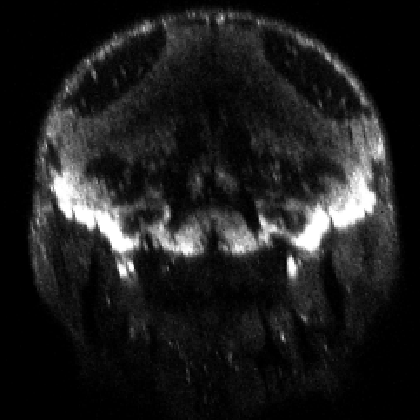
\includegraphics[width=\textwidth]{\Images/hu_grad_roaw.png}
    \end{subfigure}
    \begin{subfigure}[b]{0.2245\textwidth}
        \caption{
        Vérité terrain
            }
       \centering 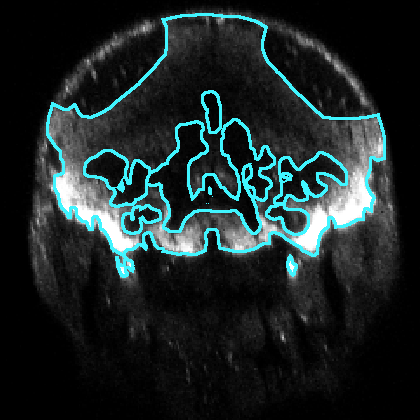
\includegraphics[width=\textwidth]{\Images/hu_grad_gt.png}
    \end{subfigure}
    \begin{subfigure}[b]{0.2245\textwidth}
        \caption{
            \centering{
                Segmentation automatique
                }
            }
       \centering 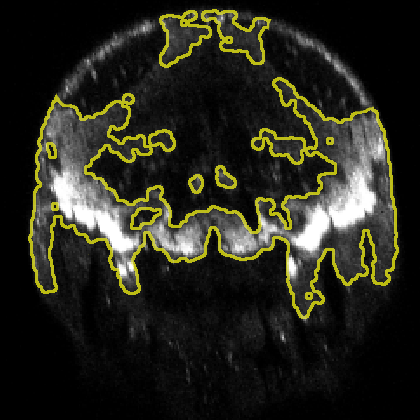
\includegraphics[width=\textwidth]{\Images/hu_grad_seuillage.png}
    \end{subfigure}
    \begin{subfigure}[b]{0.2245\textwidth}
        \caption{
            Comparaison
            }
       \centering 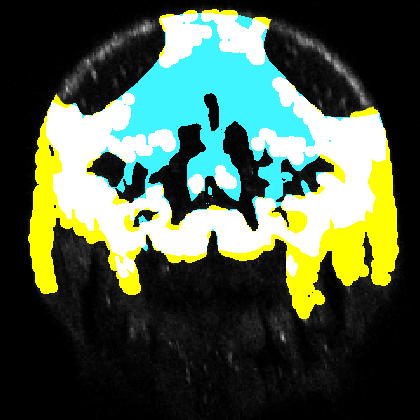
\includegraphics[width=\textwidth]{\Images/hu_grad_sup.png}
    \end{subfigure}
    \caption{
    \label{apriori:grad}
        Résultat de segmentation sur une coupe transversale d'un échantillon de \pz{} à 5dpf marquée par anticorps anti\hyp{}HuC/D et acquise en microscopie confocale.
        \newline
        La présence d'un important défaut de marquage peut entraîner simultanément une sous-segmentation et une sur\hyp{}segmentation. Ce défaut peut ainsi compromettre la distinction entre le fond et l'objet d'intérêt.
        Cet exemple montre qu'un marquage insuffisamment contrasté ne peut être segmenté correctement par la machine alors qu'un opérateur humain est mesure d'effectuer une segmentation correcte en utilisant ses connaissances.
        \newline
        Les pixels cyan, jaune et blanc représentent respectivement une segmentation manuelle considérée comme la vérité de terrain,
        le résultat de la segmentation automatique et la superposition entre les deux.
    }
\end{center}
\end{figure}

Dans ces deux cas, les méthodes de segmentations basées sur une différence de valeur de gris seront incapables de déterminer efficacement la position de l'objet d'intérêt.
%
De plus, s'il n'est pas possible de fournir d'autres caractéristiques à la segmentation, la détection de l'objet d'intérêt sera impossible sans pré\hyp{}traitement des images obtenues.

%
Nous allons donc maintenant voir différentes approches ayant été proposées pour compenser de potentiels défauts de contraste au sein d'image.

\end{document}
